\section{THPT Hai Bà Trưng 25--26, Lần 1}
\caulc
\Opensolutionfile{ans}[ans/ans-69-26-2-Hue-HaiBaTrung-L2-LC]
\begin{ex} % [Câu 1 - Mức độ Nhận biết]
	Tìm nguyên hàm của hàm số $f(x)=x^{2}-\dfrac{2}{x^{2}}$.
	\choice
	{\True $\int f(x)\,\text{d}x=\dfrac{x^{3}}{3}+\dfrac{2}{x}+C$}
	{$\int f(x)\,\text{d}x=\dfrac{x^{3}}{3}-\dfrac{2}{x}+C$}
	{$\int f(x)\,\text{d}x=\dfrac{x^{3}}{3}+\dfrac{1}{x}+C$}
	{$\int f(x)\,\text{d}x=\dfrac{x^{3}}{3}-\dfrac{1}{x}+C$}
	\loigiai{
		Ta có $\int f(x)\,\text{d}x = \int \left(x^{2}-\dfrac{2}{x^{2}}\right)\,\text{d}x = \dfrac{x^3}{3} - 2\left(-\dfrac{1}{x}\right) + C = \dfrac{x^3}{3} + \dfrac{2}{x} + C$.
		\\ \textbf{Chọn A.}
	}
\end{ex}

\begin{ex} % [Câu 2 - Mức độ Thông hiểu]
	Cho cấp số nhân $(u_{n})$ với $u_{1}=2$ và $u_{2}=6$. Giá trị của $u_{3}$ bằng
	\choice
	{$3$}
	{$24$}
	{\True $18$}
	{$10$}
	\loigiai{
		Công bội của cấp số nhân là $q = \dfrac{u_2}{u_1} = \dfrac{6}{2} = 3$.
		\\ Giá trị của $u_3$ là $u_3 = u_1 \cdot q^2 = 2 \cdot 3^2 = 18$.
		\\ \textbf{Chọn C.}
	}
\end{ex}

\begin{ex} % [Câu 3 - Mức độ Nhận biết]
	Trong không gian $Oxyz$, cho hai điểm $A(3;-2;3)$ và $B(-1;2;5)$. Tìm tọa độ trung điểm $I$ của đoạn thẳng $AB$.
	\choice
	{$I(2;-2;-1)$}
	{$I(-2;2;1)$}
	{$I(2;0;8)$}
	{\True $I(1;0;4)$}
	\loigiai{
		Tọa độ trung điểm $I$ của $AB$ được tính bởi công thức:
		\[ \begin{cases} x_I = \dfrac{x_A + x_B}{2} = \dfrac{3 + (-1)}{2} = 1 \\ y_I = \dfrac{y_A + y_B}{2} = \dfrac{-2 + 2}{2} = 0 \\ z_I = \dfrac{z_A + z_B}{2} = \dfrac{3 + 5}{2} = 4 \end{cases} \Rightarrow I(1;0;4). \]
		\textbf{Chọn D.}
	}
\end{ex}

\begin{ex} % [Câu 4 - Mức độ Nhận biết]
	Tập nghiệm của phương trình $\tan x=\sqrt{3}$ là
	\choice
	{$S=\left\{\dfrac{\pi}{6}+k\pi \mid k\in \mathbb{Z}\right\}$}
	{$S=\left\{\dfrac{\pi}{6}+k2\pi \mid k\in \mathbb{Z}\right\}$}
	{$S=\left\{\dfrac{\pi}{3}+k2\pi \mid k\in \mathbb{Z}\right\}$}
	{\True $S=\left\{\dfrac{\pi}{3}+k\pi \mid k\in \mathbb{Z}\right\}$}
	\loigiai{
		Ta có $\tan x = \sqrt{3} \Leftrightarrow \tan x = \tan \dfrac{\pi}{3} \Leftrightarrow x = \dfrac{\pi}{3} + k\pi \quad (k \in \mathbb{Z})$.
		\\ Tập nghiệm của phương trình là $S=\left\{\dfrac{\pi}{3}+k\pi \mid k\in \mathbb{Z}\right\}$.
		\\ \textbf{Chọn D.}
	}
\end{ex}

\begin{ex} % [Câu 5 - Mức độ Thông hiểu]
	Cho hàm số $f(x)$ liên tục trên $\mathbb{R}$. Gọi $S$ là diện tích hình phẳng giới hạn bởi các đường $y=f(x)$, $y=0$, $x=-1$ và $x=4$. Mệnh đề nào dưới đây đúng?
	\begin{center}
		\begin{tikzpicture}[scale=0.8, font=\footnotesize, line join=round, line cap=round, >=stealth]
			\draw[->] (-2.5,0)--(5.5,0) node[below] {$x$};
			\draw[->] (0,-2.5)--(0,2.5) node[left] {$y$};
			\fill (0,0) circle (1.5pt) node[below left] {$O$};
			\draw[smooth, samples=150, domain=-1.5:4.4, thick] plot (\x, {0.25*(\x+1)*(\x-1)*(\x-4)}) node[left] {$y=f(x)$};
			\fill[pattern=north east lines, pattern color=black] (-1,0) -- plot[domain=-1:1] (\x, {0.25*(\x+1)*(\x-1)*(\x-4)}) -- (1,0) -- cycle;
			\fill[pattern=north east lines, pattern color=black] (1,0) -- plot[domain=1:4] (\x, {0.25*(\x+1)*(\x-1)*(\x-4)}) -- (4,0) -- cycle;
			\node[below left] at (-1,0) {$-1$};
			\node[below] at (1,0) {$1$};
			\node[below right] at (4,0) {$4$};
		\end{tikzpicture}
	\end{center}
	\choice
	{$\displaystyle S=-\int_{-1}^{1}f(x)\,\text{d}x+\int_{1}^{4}f(x)\,\text{d}x$}
	{$\displaystyle  S=-\int_{-1}^{1}f(x)\,\text{d}x-\int_{1}^{4}f(x)\,\text{d}x$}
	{$\displaystyle S=\int_{-1}^{1}f(x)\,\text{d}x+\int_{1}^{4}f(x)\,\text{d}x$}
	{\True $\displaystyle S=\int_{-1}^{1}f(x)\,\text{d}x-\int_{1}^{4}f(x)\,\text{d}x$}
	\loigiai{
		Dựa vào đồ thị, trên đoạn $[-1;1]$ thì $f(x) \ge 0$, và trên đoạn $[1;4]$ thì $f(x) \le 0$.
		\\ Diện tích hình phẳng $S$ được tính bằng:
		\[ S = \int_{-1}^{4} |f(x)|\,\text{d}x = \int_{-1}^{1} f(x)\,\text{d}x - \int_{1}^{4} f(x)\,\text{d}x. \]
		\textbf{Chọn D.}
	}
\end{ex}

\begin{ex} % [Câu 6 - Mức độ Thông hiểu]
	Trong không gian $Oxyz$, cho hai điểm $A(0;0;1)$ và $B(2;1;3)$. Mặt phẳng đi qua $A$ và vuông góc với $AB$ có phương trình là
	\choice
	{\True $2x+y+2z-2=0$}
	{$2x+y+4z-4=0$}
	{$2x+y+4z-17=0$}
	{$2x+y+2z-11=0$}
	\loigiai{
		Mặt phẳng $(\alpha)$ vuông góc với đường thẳng $AB$ nên nhận vectơ $\vec{AB} = (2;1;2)$ làm một vectơ pháp tuyến.
		\\ Phương trình mặt phẳng $(\alpha)$ đi qua $A(0;0;1)$ là:
		\[ 2(x-0) + 1(y-0) + 2(z-1) = 0 \Leftrightarrow 2x+y+2z-2=0. \]
		\textbf{Chọn A.}
	}
\end{ex}

\begin{ex} % [Câu 7 - Mức độ Thông hiểu]
	\immini{
	Cho hình lập phương $ABCD.A'B'C'D'$. Góc giữa hai đường thẳng $BA'$ và $CD$ bằng
	}{
		\begin{tikzpicture}[scale=1.5, font=\footnotesize, line join=round, line cap=round, >=stealth]
			\coordinate (A) at (0,0);
			\coordinate (B) at (2,0);
			\coordinate (D) at (-0.6,-0.6);
			\coordinate (C) at ($(B)+(D)-(A)$);
			\coordinate (A') at ($(A)+(0,2)$);
			\coordinate (B') at ($(B)+(0,2)$);
			\coordinate (C') at ($(C)+(0,2)$);
			\coordinate (D') at ($(D)+(0,2)$);
			\draw[dashed, thin] (A)--(B) (A)--(D) (A)--(A');
			\draw[thick] (B)--(C)--(D) (B)--(B') (C)--(C') (D)--(D') (A')--(B')--(C')--(D')--cycle;
			\draw[dashed, thick, blue] (B)--(A');
			\node[above right] at (A) {$A$};
			\node[below right] at (B) {$B$};
			\node[below right] at (C) {$C$};
			\node[below left] at (D) {$D$};
			\node[above right] at (A') {$A'$};
			\node[above right] at (B') {$B'$};
			\node[above left] at (C') {$C'$};
			\node[above left] at (D') {$D'$};
		\end{tikzpicture}
	}
	\choice
	{$90^\circ$}
	{$60^\circ$}
	{\True $45^\circ$}
	{$30^\circ$}
	\loigiai{
		Trong hình lập phương $ABCD.A'B'C'D'$, ta có $CD \parallel AB$.
		\\ Do đó, góc giữa hai đường thẳng $BA'$ và $CD$ chính là góc giữa hai đường thẳng $BA'$ và $AB$, tức là góc $\widehat{A'BA}$.
		\\ Xét tam giác vuông $A'AB$ có $A'A = AB$ (cạnh hình lập phương) nên $\Delta A'AB$ vuông cân tại $A$.
		\\ Suy ra $\widehat{A'BA} = 45^\circ$.
		\\ \textbf{Chọn C.}
	}
\end{ex}

\begin{ex} % [Câu 8 - Mức độ Vận dụng]
	Khảo sát thời gian chơi thể thao trong một ngày của $40$ học sinh lớp 12A, giáo viên thu được mẫu số liệu ghép nhóm như sau:
	\begin{center}
		\begin{tabular}{|l|c|c|c|c|c|c|}
			\hline
			Thời gian (phút) & $[30;40)$ & $[40;50)$ & $[50;60)$ & $[60;70)$ & $[70;80)$ & $[80;90)$ \\
			\hline
			Số học sinh & $2$ & $10$ & $16$ & $8$ & $2$ & $2$ \\
			\hline
		\end{tabular}
	\end{center}
	Khoảng tứ phân vị của mẫu số liệu ghép nhóm trên là
	\choice
	{$\Delta_Q = 14$}
	{\True $\Delta_Q = 14,5$}
	{$\Delta_Q = 17$}
	{$\Delta_Q = 17,5$}
	\loigiai{
		Cỡ mẫu $n=40$. Ta tính tần số tích lũy:
		\\ Nhóm 1: $2$; Nhóm 2: $12$; Nhóm 3: $28$; Nhóm 4: $36$; Nhóm 5: $38$; Nhóm 6: $40$.
		\\ Tứ phân vị thứ nhất $Q_1$ thuộc nhóm $[40;50)$ (vì $\dfrac{40}{4}=10 \in (2;12]$).
		\[ Q_1 = 40 + \dfrac{10 - 2}{10} \cdot 10 = 48. \]
		Tứ phân vị thứ ba $Q_3$ thuộc nhóm $[60;70)$ (vì $\dfrac{3 \cdot 40}{4}=30 \in (28;36]$).
		\[ Q_3 = 60 + \dfrac{30 - 28}{8} \cdot 10 = 62,5. \]
		Khoảng tứ phân vị là $\Delta_Q = Q_3 - Q_1 = 62,5 - 48 = 14,5$.
		\\ \textbf{Chọn B.}
	}
\end{ex}

\begin{ex} % [Câu 9 - Mức độ Thông hiểu]
	Nghiệm của phương trình $\log_{2}(x+3)=5$ là
	\choice
	{$x=35$}
	{\True $x=29$}
	{$x=7$}
	{$x=13$}
	\loigiai{
		Điều kiện xác định: $x+3 > 0 \Leftrightarrow x > -3$.
		\\ Phương trình đã cho tương đương với:
		\[ x+3 = 2^5 \Leftrightarrow x+3 = 32 \Leftrightarrow x = 29 \text{ (thỏa mãn)}. \]
		Vậy nghiệm của phương trình là $x=29$.
		\\ \textbf{Chọn B.}
	}
\end{ex}

\begin{ex} % [Câu 10 - Mức độ Nhận biết]
	Trong không gian $Oxyz$, đường thẳng $d:\dfrac{x+3}{1}=\dfrac{y-1}{-1}=\dfrac{z-5}{2}$ có một vectơ chỉ phương là
	\choice
	{\True $\vec{u_{1}}=(1;-1;2)$}
	{$\vec{u_{2}}=(1;-1;-2)$}
	{$\vec{u_{3}}=(3;-1;5)$}
	{$\vec{u_{4}}=(-3;1;5)$}
	\loigiai{
		Từ phương trình chính tắc của đường thẳng $d:\dfrac{x-x_0}{a}=\dfrac{y-y_0}{b}=\dfrac{z-z_0}{c}$, ta có vectơ chỉ phương của $d$ là $\vec{u} = (a;b;c)$.
		\\ Suy ra một vectơ chỉ phương của $d$ là $\vec{u_{1}}=(1;-1;2)$.
		\\ \textbf{Chọn A.}
	}
\end{ex}

\begin{ex} % [Câu 11 - Mức độ Nhận biết]
	Đường tiệm cận đứng của đồ thị hàm số $y=\dfrac{2x-3}{x+1}$ có phương trình là
	\choice
	{$x=1$}
	{$y=2$}
	{\True $x=-1$}
	{$y=-3$}
	\loigiai{
		Hàm số đã cho có tập xác định $D = \mathbb{R} \setminus \{-1\}$.
		\\ Ta có $\lim\limits_{x \to -1^+} y = -\infty$ và $\lim\limits_{x \to -1^-} y = +\infty$.
		\\ Vậy đồ thị hàm số có đường tiệm cận đứng là $x=-1$.
		\\ \textbf{Chọn C.}
	}
\end{ex}

\begin{ex} % [Câu 12 - Mức độ Thông hiểu]
	\immini{
	Cho khối chóp $S.ABC$ có đáy $ABC$ là tam giác vuông cân tại $B$ và $AC=a\sqrt{2}$, cạnh bên $SA$ vuông góc với mặt phẳng đáy và $SA=a$. Tính thể tích $V$ của khối chóp đã cho.
	}{
		\begin{tikzpicture}[scale=1, font=\footnotesize, line join=round, line cap=round, >=stealth]
			\coordinate (B) at (-1,-1.5);
			\coordinate (A) at (-1.5,-1);
			\coordinate (C) at (2.5,-1);
			\coordinate (S) at ($(A)+(0,3)$);
			\draw[dashed, thin] (A)--(C);
			\draw[thick] (S)--(A)--(B)--(C)--cycle (S)--(B);
			\node[above] at (S) {$S$};
			\node[below left] at (A) {$A$};
			\node[below] at (B) {$B$};
			\node[below right] at (C) {$C$};
			\pic[draw, angle radius=2.5mm] {right angle=S--A--B};
			\pic[draw, angle radius=2.5mm] {right angle=S--A--C};
			\pic[draw, angle radius=2.5mm] {right angle=A--B--C};
		\end{tikzpicture}
	}
	\choice
	{$V=a^{3}$}
	{\True $V=\dfrac{a^{3}}{6}$}
	{$V=\dfrac{a^{3}}{3}$}
	{$V=\dfrac{a^{3}}{2}$}
	\loigiai{
		Đáy $ABC$ là tam giác vuông cân tại $B$, có cạnh huyền $AC=a\sqrt{2}$ nên:
		\[ AB = BC = \dfrac{AC}{\sqrt{2}} = \dfrac{a\sqrt{2}}{\sqrt{2}} = a. \]
		Diện tích đáy $S_{\Delta ABC} = \dfrac{1}{2}AB \cdot BC = \dfrac{1}{2}a^2$.
		\\ Vì $SA \perp (ABC)$ nên $SA$ là chiều cao của khối chóp, $h = SA = a$.
		\\ Thể tích khối chóp là $V = \dfrac{1}{3} \cdot S_{\Delta ABC} \cdot SA = \dfrac{1}{3} \cdot \dfrac{1}{2}a^2 \cdot a = \dfrac{a^3}{6}$.
		\\ \textbf{Chọn B.}
	}
\end{ex}
\Closesolutionfile{ans}
\cauds
\Opensolutionfile{ans}[ans/ans-69-26-2-Hue-HaiBaTrung-L2-DS]
\begin{ex} % [Câu 1 - Mức độ Vận dụng]
	\immini{
	Trên mặt đất bằng phẳng có ba chiếc cọc thẳng đứng, với ba chân cọc $A, B, C$ tạo thành một tam giác vuông cân tại $A$ và $AB=60\text{ cm}$. Ba đỉnh cọc $A', B', C'$ có độ cao lần lượt là $50\text{ cm}$, $50\text{ cm}$ và $120\text{ cm}$. Phía trên đầu cọc, người ta đặt một quả cầu trang trí sao cho mặt cầu đi qua cả ba đỉnh $A', B', C'$. 
	Chọn hệ trục tọa độ $Oxyz$ sao cho $A$ là gốc tọa độ, tia $AB$ là tia $Ox$, tia $AC$ là tia $Oy$ và tia $AA'$ là tia $Oz$ (đơn vị trên mỗi trục là $\text{cm}$).
	Các mệnh đề sau đúng hay sai?
	}{
		\begin{tikzpicture}[scale=0.8, font=\footnotesize, line join=round, line cap=round, >=stealth]
			% Base
			\draw[fill=gray!10, thin] (0.5,-1) ellipse (4cm and 1.5cm);
			
			% Axes coordinates
			\coordinate (A) at (0,0);
			\coordinate (B) at (-2,-1.5);
			\coordinate (C) at (3,-0.5);
			
			% Các đỉnh cọc được tịnh tiến lên cao thêm 2 đơn vị
			\coordinate (A') at (0,4.5);
			\coordinate (B') at (-2,3);
			\coordinate (C') at (3,7.5); 
			
			% Tâm mặt cầu K cũng tịnh tiến lên 2 đơn vị tương ứng
			\coordinate (K) at (0.5, 5.25); 
			
			% Axes (kéo dài trục z để cân đối)
			\draw[->, dashed] (A) -- ($(A)!1.5!(B)$) node[left] {$x$};
			\draw[->, dashed] (A) -- ($(A)!1.3!(C)$) node[right] {$y$};
			\draw[->, dashed] (A) -- (0,9) node[above] {$z$};
			
			% Triangle ABC
			\draw[dashed, thick] (B) -- (C) -- (A) -- cycle;
			
			% Poles
			\draw[line width=3pt, black] (A) -- (A');
			\draw[line width=3pt, black] (B) -- (B');
			\draw[line width=3pt, black] (C) -- (C');
			
			% Sphere (Đổi màu nhẹ hơn thành gray!10 và tăng độ trong suốt)
			\shade[ball color=gray!10, opacity=0.7] (K) circle (3.36);
			
			% Labels and points
			\fill (A) circle (1.5pt) node[below right] {$A$};
			\fill (B) circle (1.5pt) node[below] {$B$};
			\fill (C) circle (1.5pt) node[below] {$C$};
			
			\fill (A') circle (1.5pt) node[below right] {$A'$};
			\fill (B') circle (1.5pt) node[left] {$B'$};
			\fill (C') circle (1.5pt) node[right] {$C'$};
		\end{tikzpicture}
	}
	\choiceTF
	{$A'(0;0;120)$}
	{Đường thẳng $A'C'$ tạo với mặt đất một góc $41^\circ$ (làm tròn kết quả đến hàng đơn vị)}
	{\True Mặt phẳng $(A'BC)$ có phương trình $5x+5y+6z-300=0$}
	{\True Người ta muốn thay quả cầu hiện tại bằng một quả cầu mới có kích thước nhỏ nhất có thể sao cho mặt cầu này vẫn chạm được vào cả ba đỉnh cọc $A', B', C'$ (để không bị lọt hẳn xuống dưới). Khi đó bán kính của quả cầu mới này bằng $55\text{ cm}$}
	\loigiai{
		Theo cách chọn hệ trục tọa độ, ta xác định được tọa độ các điểm:
		\\ $A(0;0;0)$, $B(60;0;0)$, $C(0;60;0)$.
		\\ Vì $AA'=50$, $BB'=50$, $CC'=120$ nên tọa độ các đỉnh cọc là:
		\\ $A'(0;0;50)$, $B'(60;0;50)$, $C'(0;60;120)$.
		
		\begin{itemchoice}
			\itemch \textbf{Sai.} Tọa độ đúng của đỉnh cọc $A'$ là $A'(0;0;50)$.
			
			\itemch \textbf{Sai.} Ta có $\vec{A'C'} = (0; 60; 70)$. Mặt đất là mặt phẳng $(Oxy)$ có vectơ pháp tuyến $\vec{k} = (0;0;1)$.
			\\ Gọi $\alpha$ là góc giữa $A'C'$ và mặt đất, ta có:
			\[ \sin \alpha = \dfrac{|\vec{A'C'} \cdot \vec{k}|}{|\vec{A'C'}| \cdot |\vec{k}|} = \dfrac{70}{\sqrt{0^2+60^2+70^2} \cdot 1} = \dfrac{70}{10\sqrt{85}} \approx 0,759. \]
			Suy ra $\alpha \approx 49^\circ \neq 41^\circ$.
			
			\itemch \textbf{Đúng.} Mặt phẳng $(A'BC)$ đi qua $3$ điểm $A'(0;0;50)$, $B(60;0;0)$, $C(0;60;0)$.
			\\ Phương trình đoạn chắn của mặt phẳng này là:
			\[ \dfrac{x}{60} + \dfrac{y}{60} + \dfrac{z}{50} = 1 \Leftrightarrow \dfrac{5x + 5y + 6z}{300} = 1 \Leftrightarrow 5x + 5y + 6z - 300 = 0. \]
			
			\itemch \textbf{Đúng.} Quả cầu có kích thước nhỏ nhất chứa ba đỉnh $A', B', C'$ chính là mặt cầu có đường tròn lớn ngoại tiếp tam giác $A'B'C'$. Khi đó bán kính mặt cầu bằng bán kính đường tròn ngoại tiếp $\Delta A'B'C'$.
			\\ Ta có:
			\\ $A'B'^2 = (60-0)^2 + (0-0)^2 + (50-50)^2 = 3600$.
			\\ $A'C'^2 = (0-0)^2 + (60-0)^2 + (120-50)^2 = 8500$.
			\\ $B'C'^2 = (0-60)^2 + (60-0)^2 + (120-50)^2 = 12100$.
			\\ Nhận thấy $A'B'^2 + A'C'^2 = B'C'^2$, do đó $\Delta A'B'C'$ vuông tại $A'$.
			\\ Bán kính đường tròn ngoại tiếp là $R = \dfrac{B'C'}{2} = \dfrac{\sqrt{12100}}{2} = \dfrac{110}{2} = 55\text{ cm}$.
		\end{itemchoice}
	}
\end{ex}

\begin{ex} % [Câu 2 - Mức độ Thông hiểu]
	Cho hàm số $f(x) = x^4 - 8x^2 + 3$. Các mệnh đề sau đúng hay sai?
	\choiceTF
	{\True Giá trị lớn nhất của hàm số $f(x)$ trên đoạn $[1;3]$ bằng $12$}
	{\True Hàm số $f(x)$ đồng biến trên các khoảng $(-2;0)$ và $(2;+\infty)$}
	{\True Hàm số đã cho có đạo hàm là $f'(x)=4x^3-16x$}
	{Gọi $A, B, C$ là ba điểm cực trị của đồ thị hàm số đã cho. Diện tích tam giác $ABC$ bằng $16$ (đvdt)}
	\loigiai{
		Ta có hàm số $f(x) = x^4 - 8x^2 + 3$.
		\\ Tập xác định: $\mathscr{D} = \mathbb{R}$.
		\\ Đạo hàm: $f'(x) = 4x^3 - 16x$.
		\\ $f'(x) = 0 \Leftrightarrow 4x(x^2 - 4) = 0 \Leftrightarrow \left[\begin{aligned} &x = 0 \\ &x = 2 \\ &x = -2 \end{aligned}\right.$.
		
		\begin{itemchoice}
			\itemch \textbf{Đúng.} Xét hàm số trên đoạn $[1;3]$, ta có $f'(x)=0 \Leftrightarrow x=2 \in [1;3]$.
			\\ Tính các giá trị: $f(1) = 1 - 8 + 3 = -4$; $f(2) = 16 - 32 + 3 = -13$; $f(3) = 81 - 72 + 3 = 12$.
			\\ Vậy $\max\limits_{[1;3]} f(x) = 12$.
			
			\itemch \textbf{Đúng.} Bảng xét dấu của $f'(x)$:
			\\ $f'(x) > 0$ khi $x \in (-2;0) \cup (2;+\infty)$.
			\\ Do đó hàm số đồng biến trên các khoảng $(-2;0)$ và $(2;+\infty)$.
			
			\itemch \textbf{Đúng.} Đạo hàm của hàm số là $f'(x)=4x^3-16x$.
			
			\itemch \textbf{Sai.} Các điểm cực trị của đồ thị hàm số là:
			\\ $A(0; 3)$, $B(2; -13)$ và $C(-2; -13)$.
			\\ Nhận thấy $B$ và $C$ đối xứng qua trục tung. Gọi $H$ là trung điểm của $BC \Rightarrow H(0;-13)$.
			\\ $AH \perp BC$ nên $AH$ là đường cao của tam giác $ABC$.
			\\ Độ dài đáy $BC = |x_C - x_B| = |-2 - 2| = 4$.
			\\ Độ dài đường cao $AH = |y_A - y_H| = |3 - (-13)| = 16$.
			\\ Diện tích tam giác $ABC$ là $S = \dfrac{1}{2} \cdot BC \cdot AH = \dfrac{1}{2} \cdot 4 \cdot 16 = 32 \neq 16$.
		\end{itemchoice}
	}
\end{ex}

\begin{ex} % [Câu 3 - Mức độ Vận dụng]
	Một hệ thống bán lẻ nhập khẩu điện thoại từ hai nhà máy A và B. Biết rằng nhà máy A cung cấp $60\%$ số lượng, nhà máy B cung cấp $40\%$ số lượng. Tỉ lệ điện thoại đạt chuẩn của nhà máy A là $95\%$, của nhà máy B là $90\%$.
	Khi có đơn đặt hàng online, hệ thống sẽ xuất ngẫu nhiên $1$ chiếc điện thoại để giao. Quy trình xuất kho như sau: Nếu đơn hàng là giao hỏa tốc, hệ thống chỉ xuất điện thoại từ kho của nhà máy A. Còn nếu đơn hàng là giao tiêu chuẩn, hệ thống xuất ngẫu nhiên $1$ chiếc điện thoại bất kỳ trong kho chung của cả $2$ nhà máy (xác suất chọn các máy là như nhau). Biết $20\%$ đơn hàng của hệ thống là giao hỏa tốc, $80\%$ đơn hàng là giao tiêu chuẩn.
	Các mệnh đề sau đúng hay sai?
	\choiceTF
	{Xác suất để chiếc điện thoại được xuất kho thuộc nhà máy A là $0,48$}
	{Xác suất chiếc điện thoại được xuất kho là điện thoại đạt chuẩn bằng $0,744$}
	{\True Xác suất để chiếc điện thoại được xuất kho là của nhà máy B và đạt chuẩn là $0,288$}
	{Giả sử chiếc điện thoại được giao cho khách không đạt chuẩn. Xác suất để chiếc điện thoại đó do nhà máy B sản xuất là $\dfrac{17}{33}$}
	\loigiai{
		Gọi $H$ là biến cố ``Đơn hàng giao hỏa tốc'' $\Rightarrow P(H) = 0,2$.
		\\ Gọi $T$ là biến cố ``Đơn hàng giao tiêu chuẩn'' $\Rightarrow P(T) = 0,8$.
		\\ Gọi $A$ là biến cố ``Điện thoại xuất kho từ nhà máy A''.
		\\ Gọi $B$ là biến cố ``Điện thoại xuất kho từ nhà máy B''.
		\\ Gọi $C$ là biến cố ``Điện thoại được xuất kho đạt chuẩn''.
		
		Sơ đồ hình cây biểu diễn không gian mẫu và các xác suất:
		\begin{center}
			\begin{tikzpicture}[
				grow=right, 
				>=stealth, 
				edge from parent/.style={draw, -, thick},
				level distance=3.8cm,                    % Tăng chiều dài nhánh ngang để chữ có không gian "thở"
				level 1/.style={sibling distance=5.5cm}, % Tăng khoảng cách dọc giữa cụm Tiêu chuẩn & Hỏa tốc
				level 2/.style={sibling distance=2.5cm}, % Giãn cách dọc giữa Kho A & Kho B
				level 3/.style={sibling distance=1.5cm}  % Giãn cách dọc giữa Đạt & Không đạt
				]
				\node {Đơn hàng}
				child {node {Tiêu chuẩn}
					child {node {Kho B}
						child {node {Không đạt} edge from parent node[below, sloped] {\scriptsize $0,1$}}
						child {node {Đạt chuẩn} edge from parent node[above, sloped] {\scriptsize $0,9$}}
						edge from parent node[below, sloped] {\scriptsize $0,4$}
					}
					child {node {Kho A}
						child {node {Không đạt} edge from parent node[below, sloped] {\scriptsize $0,05$}}
						child {node {Đạt chuẩn} edge from parent node[above, sloped] {\scriptsize $0,95$}}
						edge from parent node[above, sloped] {\scriptsize $0,6$}
					}
					edge from parent node[below, sloped] {\scriptsize $0,8$}
				}
				child {node {Hỏa tốc}
					child {node {Kho A}
						child {node {Không đạt} edge from parent node[below, sloped] {\scriptsize $0,05$}}
						child {node {Đạt chuẩn} edge from parent node[above, sloped] {\scriptsize $0,95$}}
						edge from parent node[above, sloped] {\scriptsize $1$}}
					edge from parent node[above, sloped] {\scriptsize $0,2$}
				};
			\end{tikzpicture}
		\end{center}
		\begin{itemchoice}
			\itemch \textbf{Sai.} Xác suất để chiếc điện thoại xuất kho thuộc nhà máy A là:
			\[ P(A) = P(H) \cdot P(A|H) + P(T) \cdot P(A|T) = 0,2 \cdot 1 + 0,8 \cdot 0,6 = 0,68. \]
			Từ đó suy ra $P(B) = 1 - P(A) = 1 - 0,68 = 0,32$.
			
			\itemch \textbf{Sai.} Xác suất chiếc điện thoại được xuất kho đạt chuẩn là:
			\[ P(C) = P(A) \cdot P(C|A) + P(B) \cdot P(C|B) = 0,68 \cdot 0,95 + 0,32 \cdot 0,9 = 0,646 + 0,288 = 0,934. \]
			
			\itemch \textbf{Đúng.} Xác suất điện thoại của nhà máy B và đạt chuẩn là:
			\[ P(B \cap C) = P(B) \cdot P(C|B) = 0,32 \cdot 0,9 = 0,288. \]
			
			\itemch \textbf{Sai.} Xác suất điện thoại không đạt chuẩn là $P(\overline{C}) = 1 - P(C) = 1 - 0,934 = 0,066$.
			\\ Xác suất điện thoại không đạt chuẩn và do nhà máy B sản xuất là:
			\[ P(B \cap \overline{C}) = P(B) \cdot P(\overline{C}|B) = 0,32 \cdot (1 - 0,9) = 0,032. \]
			Giả sử điện thoại giao cho khách không đạt chuẩn, xác suất để nó do nhà máy B sản xuất là:
			\[ P(B|\overline{C}) = \dfrac{P(B \cap \overline{C})}{P(\overline{C})} = \dfrac{0,032}{0,066} = \dfrac{32}{66} = \dfrac{16}{33} \neq \dfrac{17}{33}. \]
		\end{itemchoice}
	}
\end{ex}

\begin{ex} % [Câu 4 - Mức độ Vận dụng]
	Để thúc đẩy kinh tế số, một tỉnh phê duyệt gói ngân sách $20$ tỷ đồng để xây dựng hạ tầng công nghệ cho dự án Công viên phần mềm trong vòng $20$ tháng. Gọi $t$ (tháng) là thời gian tính từ lúc bắt đầu dự án $(0 \le t \le 20)$ và $V(t)$ (triệu đồng) là số tiền còn lại chưa giải ngân tại thời điểm $t$. Biết rằng tốc độ giải ngân tại thời điểm $t$ là $V'(t) = k \cdot e^{0,1t}$, trong đó $k$ là hệ số tỉ lệ $(k < 0)$. Toàn bộ số tiền $20$ tỷ đồng được giải ngân vừa hết sau đúng $20$ tháng.
	Các mệnh đề sau đúng hay sai?
	\choiceTF
	{\True $V(t)$ là một nguyên hàm của hàm số $V'(t) = k \cdot e^{0,1t}$}
	{Sau $10$ tháng, số tiền còn lại chưa giải ngân là $5,4$ tỷ đồng (làm tròn kết quả đến hàng phần chục)}
	{\True Hệ số tỉ lệ $k = \dfrac{2000}{1-e^2}$}
	{Có duy nhất một thời điểm $t_0 \in (0;20)$ mà tại đó tốc độ giải ngân đúng bằng tốc độ giải ngân trung bình của cả dự án. Khi đó $t_0 > 12$}
	\loigiai{
		Ta có hàm số $V(t)$ là số tiền còn lại chưa giải ngân (tính theo triệu đồng).\\
		Số tiền ban đầu là $20$ tỷ đồng $= 20000$ triệu đồng.
		\\ Theo giả thiết, $V(0) = 20000$ và $V(20) = 0$.
		
		\begin{itemchoice}
			\itemch \textbf{Đúng.} Theo định nghĩa, hàm số $V(t)$ là một nguyên hàm của hàm tốc độ thay đổi $V'(t)$.
			\\ Ta có: $V(t) = \int V'(t)\,\text{d}t = \int k \cdot e^{0,1t}\,\text{d}t = 10k \cdot e^{0,1t} + C$.
			
			\itemch \textbf{Sai.} Dựa vào các điều kiện, ta có hệ phương trình:
			\[ \begin{cases} V(0) = 20000 \\ V(20) = 0 \end{cases} \Leftrightarrow \begin{cases} 10k + C = 20000 \\ 10k \cdot e^2 + C = 0 \end{cases} \Leftrightarrow \begin{cases} C = -10k \cdot e^2 \\ 10k(1 - e^2) = 20000 \end{cases} \]
			Từ đó suy ra $k = \dfrac{2000}{1-e^2}$ (vì $1 - e^2 < 0 \Rightarrow k < 0$, thỏa mãn).
			\\ Khi đó $C = \dfrac{-20000 \cdot e^2}{1-e^2}$.
			\\ Hàm số lượng tiền còn lại là: $V(t) = \dfrac{20000}{1-e^2} \cdot e^{0,1t} - \dfrac{20000 \cdot e^2}{1-e^2} = \dfrac{20000}{1-e^2} \left( e^{0,1t} - e^2 \right)$.
			\\ Sau $10$ tháng ($t=10$), số tiền còn lại là:
			\[ V(10) = \dfrac{20000}{1-e^2}(e - e^2) = \dfrac{20000 \cdot e(1-e)}{(1-e)(1+e)} = \dfrac{20000e}{1+e} \approx 14621 \text{ (triệu đồng)}. \]
			Tức là còn lại khoảng $14,6$ tỷ đồng. Do đó khẳng định còn lại $5,4$ tỷ đồng là sai. (Thực tế $5,4$ tỷ đồng xấp xỉ số tiền \textbf{đã} giải ngân).
			
			\itemch \textbf{Đúng.} Theo kết quả đã giải ở trên, ta có hệ số tỉ lệ $k = \dfrac{2000}{1-e^2}$.
			
			\itemch \textbf{Sai.} Tốc độ giải ngân trung bình của cả dự án là:
			\[ v_{\text{tb}} = \dfrac{V(20) - V(0)}{20 - 0} = \dfrac{0 - 20000}{20} = -1000 \text{ (triệu đồng/tháng)}. \]
			Thời điểm $t_0$ mà tốc độ giải ngân đúng bằng tốc độ trung bình thỏa mãn:
			\[ V'(t_0) = -1000 \Leftrightarrow k \cdot e^{0,1t_0} = -1000 \Leftrightarrow \dfrac{2000}{1-e^2} \cdot e^{0,1t_0} = -1000 \]
			\[ \Leftrightarrow e^{0,1t_0} = \dfrac{-1000(1-e^2)}{2000} = \dfrac{e^2 - 1}{2} \approx 3,1945. \]
			\[ \Leftrightarrow 0,1t_0 = \ln\left(\dfrac{e^2 - 1}{2}\right) \Leftrightarrow t_0 = 10 \cdot \ln\left(\dfrac{e^2 - 1}{2}\right) \approx 11,61 \text{ (tháng)}. \]
			Giá trị $t_0 \approx 11,61 \notin (12; +\infty)$ nên $t_0 > 12$ là sai.
		\end{itemchoice}
	}
\end{ex}
\Closesolutionfile{ans}
\caukq
\Opensolutionfile{ans}[ans/ans-69-26-2-Hue-HaiBaTrung-L2-KQ]
\begin{ex} % [Câu 1 - Mức độ Vận dụng Cao]
	Để chuẩn bị cho lễ kỷ niệm 110 năm ngày thành lập trường THPT Hai Bà Trưng, Đoàn trường thiết kế một bảng trang trí gồm $12$ ô vuông xếp thành lưới như hình vẽ.
	\immini{Các học sinh lớp 12A4 được giao nhiệm vụ gắn các chữ cái bằng đèn led lên bảng, bao gồm: $2$ chữ H, $1$ chữ B và $3$ chữ T (viết tắt của cụm từ "Hai Bà Trưng"). Biết mỗi ô vuông chỉ gắn tối đa một chữ cái. Hỏi có bao nhiêu cách sắp xếp các chữ cái này sao cho trên bảng xuất hiện ít nhất một dòng chữ HBT (theo hàng từ trái qua phải hoặc theo cột từ trên xuống dưới) và không có hàng nào bị trống.
	}{
		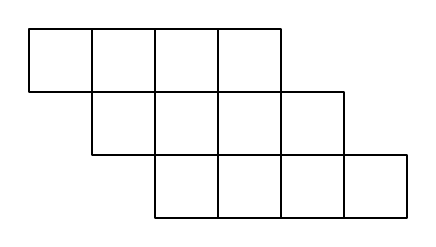
\begin{tikzpicture}[scale=0.8, line join=round, line cap=round, thick]
			% Hàng 1
			\draw (0,2) rectangle (1,3); \draw (1,2) rectangle (2,3); \draw (2,2) rectangle (3,3); \draw (3,2) rectangle (4,3);
			% Hàng 2
			\draw (1,1) rectangle (2,2); \draw (2,1) rectangle (3,2); \draw (3,1) rectangle (4,2); \draw (4,1) rectangle (5,2);
			% Hàng 3
			\draw (2,0) rectangle (3,1); \draw (3,0) rectangle (4,1); \draw (4,0) rectangle (5,1); \draw (5,0) rectangle (6,1);
		\end{tikzpicture}
	}
	\par\shortans{1642}
	\loigiai{
		\textbf{Nhận xét cốt lõi:} Bảng có $3$ hàng và $6$ cột, tổng cộng $12$ ô. Bộ chữ gồm $6$ ký tự: $2$ chữ H, $1$ chữ B, $3$ chữ T. 
		\\ Vì chỉ có duy nhất $\textbf{1}$ \textbf{chữ B}, nên trên bảng không thể có hai khối "HBT" rời rạc. Chỉ có $3$ kịch bản xảy ra: "HBT" nằm ngang, "HBT" nằm dọc, hoặc hai khối đan chéo nhau thành hình chữ thập (dùng chung chữ B).
		\begin{center}
			\begin{tikzpicture}[scale=0.65, line join=round, line cap=round, thick]
				% ====== TRƯỜNG HỢP 1: GIAO TẠI CỘT 3 ======
				\begin{scope}[xshift=0cm]
					% Vẽ khung lưới chìm
					\draw[gray!50, thin] (0,2) rectangle (1,3); \draw[gray!50, thin] (1,2) rectangle (2,3); \draw[gray!50, thin] (2,2) rectangle (3,3); \draw[gray!50, thin] (3,2) rectangle (4,3);
					\draw[gray!50, thin] (1,1) rectangle (2,2); \draw[gray!50, thin] (2,1) rectangle (3,2); \draw[gray!50, thin] (3,1) rectangle (4,2); \draw[gray!50, thin] (4,1) rectangle (5,2);
					\draw[gray!50, thin] (2,0) rectangle (3,1); \draw[gray!50, thin] (3,0) rectangle (4,1); \draw[gray!50, thin] (4,0) rectangle (5,1); \draw[gray!50, thin] (5,0) rectangle (6,1);
					
					% Tô màu và điền chữ khối DỌC
					\fill[cyan!20] (2,2) rectangle (3,3); \node at (2.5,2.5) {\textbf{H}};
					\fill[green!30] (2,1) rectangle (3,2); \node at (2.5,1.5) {\textbf{B}};
					\fill[cyan!20] (2,0) rectangle (3,1); \node at (2.5,0.5) {\textbf{T}};
					
					% Tô màu và điền chữ khối NGANG
					\fill[yellow!30] (1,1) rectangle (2,2); \node at (1.5,1.5) {\textbf{H}};
					\fill[yellow!30] (3,1) rectangle (4,2); \node at (3.5,1.5) {\textbf{T}};
					
					% Viền đậm lại hình chữ thập
					\draw[thick] (2,0) rectangle (3,3); % Cột dọc
					\draw[thick] (1,1) rectangle (4,2); % Hàng ngang
					\draw[thick] (2,1) rectangle (3,2); % Ô vuông chữ B trung tâm
					
					\node[below] at (3,-0.5) {Hình 1: Chữ thập tại Cột 3};
				\end{scope}
				
				% ====== TRƯỜNG HỢP 2: GIAO TẠI CỘT 4 ======
				\begin{scope}[xshift=8cm]
					% Vẽ khung lưới chìm
					\draw[gray!50, thin] (0,2) rectangle (1,3); \draw[gray!50, thin] (1,2) rectangle (2,3); \draw[gray!50, thin] (2,2) rectangle (3,3); \draw[gray!50, thin] (3,2) rectangle (4,3);
					\draw[gray!50, thin] (1,1) rectangle (2,2); \draw[gray!50, thin] (2,1) rectangle (3,2); \draw[gray!50, thin] (3,1) rectangle (4,2); \draw[gray!50, thin] (4,1) rectangle (5,2);
					\draw[gray!50, thin] (2,0) rectangle (3,1); \draw[gray!50, thin] (3,0) rectangle (4,1); \draw[gray!50, thin] (4,0) rectangle (5,1); \draw[gray!50, thin] (5,0) rectangle (6,1);
					
					% Tô màu và điền chữ khối DỌC
					\fill[cyan!20] (3,2) rectangle (4,3); \node at (3.5,2.5) {\textbf{H}};
					\fill[green!30] (3,1) rectangle (4,2); \node at (3.5,1.5) {\textbf{B}};
					\fill[cyan!20] (3,0) rectangle (4,1); \node at (3.5,0.5) {\textbf{T}};
					
					% Tô màu và điền chữ khối NGANG
					\fill[yellow!30] (2,1) rectangle (3,2); \node at (2.5,1.5) {\textbf{H}};
					\fill[yellow!30] (4,1) rectangle (5,2); \node at (4.5,1.5) {\textbf{T}};
					
					% Viền đậm lại hình chữ thập
					\draw[thick] (3,0) rectangle (4,3); % Cột dọc
					\draw[thick] (2,1) rectangle (5,2); % Hàng ngang
					\draw[thick] (3,1) rectangle (4,2); % Ô vuông chữ B trung tâm
					
					\node[below] at (3,-0.5) {Hình 2: Chữ thập tại Cột 4};
				\end{scope}
			\end{tikzpicture}
		\end{center}
		\textbf{Bước 1: Đếm số cách xếp khối "HBT" nằm NGANG}
		\\ - Bảng có $3$ hàng, mỗi hàng có $4$ ô liên tiếp nên có $2$ vị trí để đặt chữ "HBT" (ở $3$ ô đầu hoặc $3$ ô cuối).
		\\ $\Rightarrow$ Có tổng cộng $3 \times 2 = 6$ vị trí ngang.
		\\ - Cố định khối "HBT" vào $1$ vị trí ngang (ví dụ ở Hàng 1). Ta còn lại $9$ ô trống và phải xếp $3$ chữ còn dư ($1$ chữ H, $2$ chữ T).
		\\ - Xếp ngẫu nhiên $3$ chữ vào $9$ ô: Chọn $1$ ô cho chữ H ($C_9^1$), chọn $2$ ô cho chữ T ($C_8^2$) $\Rightarrow$ Có $C_9^1 \cdot C_8^2 = 252$ cách.
		\\ - \textit{Loại trừ trường hợp vi phạm "có hàng trống":}
		Vì Hàng 1 đã có chữ, ta chỉ lo Hàng 2 hoặc Hàng 3 bị trống.
		\begin{itemize}
			\item Nếu Hàng 2 trống: $3$ chữ còn lại bị ép chui vào $5$ ô (gồm $4$ ô Hàng 3 và $1$ ô dư Hàng 1). Có $C_5^1 \cdot C_4^2 = 30$ cách.
			\item Nếu Hàng 3 trống: Tương tự, $3$ chữ chui vào $5$ ô của Hàng 2 và Hàng 1. Có $C_5^1 \cdot C_4^2 = 30$ cách.
			\item (Không thể có trường hợp cả Hàng 2 và 3 cùng trống vì $3$ chữ không thể chui vừa $1$ ô dư của Hàng 1).
		\end{itemize}
		$\Rightarrow$ Số cách hợp lệ cho 1 vị trí ngang là: $252 - 30 - 30 = 192$ cách.
		\\ Tổng số cách ở Bước 1 là: $6 \times 192 = \textbf{1152}$ cách.
		
		\textbf{Bước 2: Đếm số cách xếp khối "HBT" nằm DỌC}
		\\ - Chỉ có Cột 3 và Cột 4 là có đủ $3$ ô dọc. Vậy có $2$ vị trí đặt "HBT" dọc.
		\\ - Khi đặt "HBT" dọc, nó đã trải dài và chiếm mỗi hàng $1$ ô. Do đó, \textbf{chắc chắn $3$ hàng đều đã có chữ (không thể bị trống)}.
		\\ - Ta chỉ việc thoải mái xếp $3$ chữ còn dư vào $9$ ô trống: $C_9^1 \cdot C_8^2 = 252$ cách.
		\\ Tổng số cách ở Bước 2 là: $2 \times 252 = \textbf{504}$ cách.
		
		\textbf{Bước 3: Trừ đi phần giao nhau (Đếm lặp)}
		- Nếu một cách xếp có cả "HBT" ngang và dọc, chúng phải cắt nhau tại chữ B. Để giao nhau được, chữ B bắt buộc phải nằm ở Hàng 2 (tại Cột 3 hoặc Cột 4).
		\\ $\Rightarrow$ Có đúng $2$ khung hình chữ thập.
		\\ - Mỗi hình chữ thập đã dùng $5$ chữ ($2$ chữ H, $1$ chữ B, $2$ chữ T) và chiếm $5$ ô (hiển nhiên $3$ hàng đều không trống).
		\\ - Ta chỉ còn dư đúng $1$ chữ T và $7$ ô trống trên bảng $\Rightarrow$ Xếp chữ T vào có $7$ cách.
		\\ Số cách bị đếm trùng là: $2 \times 7 = \textbf{14}$ cách.
		
		\textbf{Kết luận:} Áp dụng nguyên lý bù trừ, tổng số cách sắp xếp thỏa mãn yêu cầu bài toán là:
		\[ 1152 + 504 - 14 = \mathbf{1642} \text{ (cách).} \]
	}
\end{ex}

\begin{ex} % [Câu 2 - Mức độ Vận dụng]
	Một khu công viên dự định thiết kế một bồn hoa nghệ thuật có ranh giới là một tam giác đều $ABC$ với cạnh dài $6\text{ m}$. Bên trong bồn hoa, người ta xây hai bờ kè phân cách có hình dạng là hai đường parabol bằng nhau đi qua $B$ và $C$, có trục đối xứng lần lượt song song với $BA$ và $CA$. Hai bờ kè này giao nhau tại một đài phun nước ở vị trí $D$. Biết rằng đường mép $BC$ của bồn hoa tiếp xúc với cả hai đường bờ kè parabol này và khoảng cách từ đỉnh $A$ của bồn hoa đến đài phun nước $D$ là $1,4\text{ m}$. Phần diện tích giới hạn bởi hai bờ kè parabol và đoạn $BC$ (phần tô màu đen) được dùng để trồng hoa hồng. Tính diện tích phần đất trồng hoa hồng theo đơn vị $\text{m}^2$ (làm tròn kết quả đến hàng phần chục).
	\begin{center}
		\begin{tikzpicture}[scale=1.2, line join=round, line cap=round, >=stealth]
			% Khai báo các hằng số toán học chính xác (Tối ưu hóa bằng phương trình tham số Bezier bậc 2)
			\def\hA{5.19615} % Tung độ điểm A: 3*sqrt(3)
			\def\hD{3.79615} % Tung độ điểm D: 3*sqrt(3) - 1.4
			\def\xone{0.40415} % Hoành độ điểm kiểm soát P1 để trục đối xứng // BA
			
			% Tọa độ các đỉnh
			\coordinate (B) at (0,0);
			\coordinate (C) at (6,0);
			\coordinate (A) at (3,\hA);
			\coordinate (D) at (3,\hD);
			
			% Tô màu phần diện tích đen trồng hoa (hạ tone xuống xám để làm nổi bật nét bờ kè)
			\fill[pattern=north east lines, pattern color=gray!80]
			(B) --
			plot[domain=0:1, smooth, variable=\t, samples=100] ({2*\xone*\t*(1-\t) + 3*\t*\t}, {\hD*\t*\t}) --
			plot[domain=1:0, smooth, variable=\t, samples=100] ({6 - (2*\xone*\t*(1-\t) + 3*\t*\t)}, {\hD*\t*\t}) -- cycle;
			
			% Vẽ viền tam giác
			\draw[thick] (A) -- (B) -- (C) -- cycle;
			
			% Vẽ hai bờ kè Parabol bằng đường cong tham số tuyệt đối chính xác
			\draw[line width=1.2pt] plot[domain=0:1, smooth, variable=\t, samples=100] ({2*\xone*\t*(1-\t) + 3*\t*\t}, {\hD*\t*\t});
			\draw[line width=1.2pt] plot[domain=0:1, smooth, variable=\t, samples=100] ({6 - (2*\xone*\t*(1-\t) + 3*\t*\t)}, {\hD*\t*\t});
			
			% Các nét gióng và ghi chú kích thước 1.4m
			\draw[dashed, thin] (A) -- (3,0);
			\draw[dashed, thin] (A) -- (3.8,\hA);
			\draw[dashed, thin] (D) -- (3.8,\hD);
			\draw[<->, thin] (3.6, \hA) -- (3.6, \hD) node[midway, right] {$1,4\text{ m}$};
			
			% Ký hiệu kích thước 6m dưới đáy BC bằng ngoặc ôm (brace)
			\draw[decoration={brace,amplitude=5pt,mirror}, decorate, thin] 
			(0,-0.2) -- (6,-0.2) node[midway, below=5pt] {$6\text{ m}$};
			
			% Nhãn các điểm
			\fill (A) circle (1.5pt) node[above] {$A$};
			\fill (B) circle (1.5pt) node[below left] {$B$};
			\fill (C) circle (1.5pt) node[below right] {$C$};
			\fill (D) circle (1.5pt) node[above left=1pt, fill=white, inner sep=0.5pt] {$D$};
		\end{tikzpicture}
	\end{center}
	\par\shortans{10,4}
	\loigiai{
		Tam giác $ABC$ đều cạnh $6$, chiều cao tương ứng là $h_a = \dfrac{6\sqrt{3}}{2} = 3\sqrt{3}$.
		Gắn hệ trục tọa độ sao cho $B \equiv O(0;0)$, tia $BC$ là trục $Ox$, đường cao hạ từ $B$ vuông góc $BC$ là trục $Oy$.
		\begin{center}
			\begin{tikzpicture}[scale=1, line join=round, line cap=round, >=stealth]
				% Khai báo hằng số
				\def\hA{5.19615} % 3*sqrt(3)
				\def\hD{3.79615} % 3*sqrt(3) - 1.4
				\def\xone{0.40415}
				
				% Tọa độ các điểm
				\coordinate (B) at (0,0);
				\coordinate (C) at (6,0);
				\coordinate (A) at (3,\hA);
				\coordinate (D) at (3,\hD);
				
				% Tô màu phần diện tích bồn hoa
				\fill[pattern=north east lines, pattern color=gray!50]
				(B) --
				plot[domain=0:1, smooth, variable=\t, samples=100] ({2*\xone*\t*(1-\t) + 3*\t*\t}, {\hD*\t*\t}) --
				plot[domain=1:0, smooth, variable=\t, samples=100] ({6 - (2*\xone*\t*(1-\t) + 3*\t*\t)}, {\hD*\t*\t}) -- cycle;
				
				% Vẽ hệ trục tọa độ Oxy
				\draw[->, thick] (-1,0) -- (7,0) node[below] {$x$};
				\draw[->, thick] (0,-1) -- (0,6.5) node[left] {$y$};
				\node[below left] at (B) {$O \equiv B$};
				
				% Vẽ tam giác đều
				\draw[thick] (A) -- (B) -- (C) -- cycle;
				
				% Vẽ hai bờ kè Parabol
				\draw[line width=1.2pt, blue] plot[domain=0:1, smooth, variable=\t, samples=100] ({2*\xone*\t*(1-\t) + 3*\t*\t}, {\hD*\t*\t});
				\draw[line width=1.2pt, blue] plot[domain=0:1, smooth, variable=\t, samples=100] ({6 - (2*\xone*\t*(1-\t) + 3*\t*\t)}, {\hD*\t*\t});
				
				% Các đường gióng tọa độ
				\draw[dashed, thin] (A) -- (3,0) node[below right] {$3$};
				\draw[dashed, thin] (D) -- (0,\hD) node[left] {$h$};
				
				% Đánh dấu và ghi nhãn các điểm
				\fill (A) circle (1.5pt) node[above right] {$A(3; 3\sqrt{3})$};
				\fill (C) circle (1.5pt) node[above right] {$C(6; 0)$};
				\fill (D) circle (1.5pt) node[above left=1pt, fill=white, inner sep=0.5pt] {$D$};
				\fill (3,0) circle (1.5pt);
				\fill (0,\hD) circle (1.5pt);
			\end{tikzpicture}
		\end{center}
		Khi đó $B(0;0)$, $C(6;0)$, $A(3; 3\sqrt{3})$.
		\\ Điểm $D$ nằm trên đường cao hạ từ $A$, cách $A$ một đoạn $1,4\text{ m}$ nên tọa độ $D(3; 3\sqrt{3} - 1,4)$.
		\\ Đặt tung độ của $D$ là $h = 3\sqrt{3} - 1,4 \approx 3,796$.
		\\ Xét Parabol đi qua $B$, do tiếp xúc với $BC$ (trục $Ox$) tại $B$ và có trục đối xứng song song với $BA$ (tạo góc $60^\circ$), phương trình tham số của Parabol có dạng:
		\[ \begin{cases} x(t) = t^2 + v_0 t \\ y(t) = \sqrt{3}t^2 \end{cases} \quad (t \ge 0) \]
		Tại điểm $D$, $y(t_D) = h \Rightarrow t_D = \sqrt{\dfrac{h}{\sqrt{3}}}$.
		\\ Và $x(t_D) = 3 \Rightarrow v_0 = \dfrac{3}{t_D} - t_D$.
		\\ Diện tích nửa phần bồn hoa (giới hạn bởi cung $BD$, $Ox$ và $x=3$) là:
		\[ S_1 = \int_0^{t_D} y(t) x'(t) \,\text{d}t = \int_0^{t_D} \sqrt{3}t^2 (2t + v_0) \,\text{d}t = \sqrt{3} \left( \dfrac{t_D^4}{2} + \dfrac{v_0 t_D^3}{3} \right). \]
		Thế $v_0 t_D = 3 - t_D^2$ vào ta được:
		\[ S_1 = \sqrt{3} t_D^2 \left( \dfrac{t_D^2}{2} + 1 - \dfrac{t_D^2}{3} \right) = \sqrt{3} \left( \dfrac{h}{\sqrt{3}} \right) \left( 1 + \dfrac{h}{6\sqrt{3}} \right) = h + \dfrac{\sqrt{3}}{18} h^2. \]
		Diện tích toàn bộ bồn hoa là $S = 2S_1 = 2h + \dfrac{\sqrt{3}}{9} h^2$.
		\\ Thay số $h = 3\sqrt{3} - 1,4 \approx 3,79615$, ta được:
		\[ S = 2(3,79615) + \dfrac{\sqrt{3}}{9} (3,79615)^2 \approx 7,5923 + 2,7733 \approx 10,3656 \text{ m}^2. \]
		Làm tròn kết quả đến hàng phần chục, ta được $10,4\text{ m}^2$.
	}
\end{ex}
\begin{ex} % [Câu 3 - Mức độ Thông hiểu/Vận dụng]
	Cho hình chóp $S.ABC$ có đáy $ABC$ là tam giác cân tại $B$ với $BA=BC=a, \widehat{ABC}=120^\circ$. Tam giác $SAC$ là tam giác đều và nằm trong mặt phẳng vuông góc với đáy. Tính số đo của góc nhị diện $[A, SB, C]$ (đơn vị độ và làm tròn kết quả đến hàng đơn vị).
	\par\shortans{123}
	\loigiai{
		\begin{center}
			\begin{tikzpicture}[scale=1.2, font=\footnotesize, line join=round, line cap=round, >=stealth]
				\coordinate (A) at (-3,0);
				\coordinate (C) at (3,0.5);
				\coordinate (B) at (1,-2);
				\coordinate (H) at ($(A)!0.5!(C)$);
				\coordinate (S) at ($(H)+(0,4.5)$);
				\coordinate (K) at ($(S)!0.45!(B)$);
				\draw[->, dashed, blue, thin] (H) -- ($(H)!1.3!(C)$) node[right] {$x$};
				\draw[->, dashed, blue, thin] (H) -- ($(H)!1.4!(B)$) node[right] {$y$};
				\draw[->, dashed, blue, thin] (H) -- ($(H)+(0,5.5)$) node[above] {$z$};
				\draw[dashed, thin] (A) -- (C) (S) -- (H) (B) -- (H);
				\draw[thick]  (A) -- (K) -- (C);
				\draw[thick] (S) -- (A) -- (B) -- (C) -- (S) -- (B);
				\pic[draw, angle radius=2mm, thin] {right angle=S--H--C};
				\pic[draw, angle radius=2mm, thin] {right angle=A--K--S};
				\node[left] at (A) {$A$};
				\node[above right] at (C) {$C$};
				\node[below left] at (B) {$B$};
				\node[left] at (S) {$S$};
				\node[above left] at (H) {$H \equiv O$};
				\node[above right] at (K) {$K$};
			\end{tikzpicture}
		\end{center}
		\textbf{Cách 1: Phương pháp hình học thuần túy}\\
		Đáy $ABC$ cân tại $B$, $\widehat{ABC}=120^\circ \Rightarrow AC = \sqrt{a^2+a^2-2a^2\cos 120^\circ} = a\sqrt{3}$.\\
		Tam giác $SAC$ đều cạnh $a\sqrt{3}$. Gọi $H$ là trung điểm $AC \Rightarrow SH \perp AC$. Vì $(SAC) \perp (ABC)$ nên $SH \perp (ABC)$ và $SH = \dfrac{\sqrt{3}}{2}AC = \dfrac{3a}{2}$.\\
		Trong $\Delta ABC$, chiều cao $BH = BC \cdot \cos 60^\circ = \dfrac{a}{2}$. Suy ra $SB = \sqrt{SH^2 + BH^2} = \dfrac{a\sqrt{10}}{2}$.\\
		Gọi $K$ là hình chiếu vuông góc của $A$ lên $SB$. Do $\Delta SAB = \Delta SCB$ (c.c.c) nên $CK \perp SB$ và $CK = AK$. Góc phẳng nhị diện cần tìm liên quan trực tiếp đến $\widehat{AKC}$.\\
		Trong $\Delta SAB$: $\cos \widehat{SBA} = \dfrac{SB^2+AB^2-SA^2}{2 \cdot SB \cdot AB} = \dfrac{1}{2\sqrt{10}} \Rightarrow \sin \widehat{SBA} = \dfrac{\sqrt{39}}{2\sqrt{10}} \Rightarrow AK = CK = AB\sin \widehat{SBA} = \dfrac{a\sqrt{39}}{2\sqrt{10}}$.\\
		Trong $\Delta AKC$: $\cos \widehat{AKC} = \dfrac{AK^2+CK^2-AC^2}{2 \cdot AK \cdot CK} = \dfrac{\dfrac{39a^2}{20} - 3a^2}{2 \cdot \dfrac{39a^2}{40}} = -\dfrac{7}{13} \Rightarrow \widehat{AKC} \approx 122,57^\circ$. Vậy góc nhị diện bằng $123^\circ$.\\
		\textbf{Cách 2: Phương pháp tọa độ hóa (Oxyz)}\\
		Chọn hệ trục $Oxyz$ với gốc $O \equiv H(0;0;0)$, các tia $Ox, Oy, Oz$ lần lượt trùng với $HC, HB, HS$ như hình vẽ. Chọn $a=2 \Rightarrow AC = 2\sqrt{3}, SH = 3, HB = 1$.\\
		Tọa độ các điểm: $H(0;0;0)$, $C(\sqrt{3}; 0; 0)$, $A(-\sqrt{3}; 0; 0)$, $B(0; 1; 0)$, $S(0; 0; 3)$.\\
		Suy ra các vectơ: $\vec{SB} = (0; 1; -3)$, $\vec{SA} = (-\sqrt{3}; 0; -3)$, $\vec{SC} = (\sqrt{3}; 0; -3)$.\\
		Áp dụng đúng định nghĩa, góc nhị diện $\alpha = [A, SB, C]$ chính là góc giữa hai vectơ pháp tuyến quy chuẩn xuất phát từ cạnh bờ $SB$ là $\vec{n_1}$ và $\vec{n_2}$:\\
		Mặt phẳng $(SAB)$ có $\vec{n_1} = [\vec{SB}, \vec{SA}] = (-3; 3\sqrt{3}; \sqrt{3})$.\\
		Mặt phẳng $(SBC)$ có $\vec{n_2} = [\vec{SB}, \vec{SC}] = (-3; -3\sqrt{3}; -\sqrt{3})$.\\
		Khi đó, ta tính trực tiếp được côsin của góc nhị diện (không cần trị tuyệt đối):\\
		$\cos \alpha = \cos(\vec{n_1}, \vec{n_2}) = \dfrac{\vec{n_1} \cdot \vec{n_2}}{|\vec{n_1}| \cdot |\vec{n_2}|} = \dfrac{(-3)(-3) + (3\sqrt{3})(-3\sqrt{3}) + (\sqrt{3})(-\sqrt{3})}{\sqrt{9+27+3} \cdot \sqrt{9+27+3}} = \dfrac{9 - 27 - 3}{39} = -\dfrac{21}{39} = -\dfrac{7}{13}$.\\
		Vì $\cos \alpha < 0$ nên góc nhị diện là góc tù, $\alpha \approx 122,57^\circ$. Làm tròn ta được $123^\circ$.
	}
\end{ex}
\begin{ex} % [Câu 4 - Mức độ Vận dụng]
	Một hợp tác xã nông nghiệp dự định đầu tư hệ thống nhà màng trồng dưa lưới công nghệ cao với tổng diện tích là $x$ (đơn vị: $1000 \text{ m}^2$). Qua khảo sát thị trường và kỹ thuật, các chỉ số tài chính được dự báo như sau:\\
	- Chi phí đầu tư ban đầu: $C(x) = 500 + 120x$ (triệu đồng).\\
	- Doanh thu dự kiến hàng năm: $R(x) = 60x - 0,5x^2$ (triệu đồng/năm).\\
	- Chi phí vận hành hàng năm: $C_1(x) = 8 + 4x + 0,1x^2$ (triệu đồng/năm).\\
	Hãy xác định diện tích $x$ (làm tròn kết quả đến hàng phần chục) để tối đa hóa tỷ lệ lợi nhuận hàng năm trên chi phí đầu tư ban đầu.
	\par\shortans{16,3}
	\loigiai{
		Lợi nhuận hàng năm của hệ thống là:
		\[ L(x) = R(x) - C_1(x) = (60x - 0,5x^2) - (8 + 4x + 0,1x^2) = -0,6x^2 + 56x - 8. \]
		Hàm số biểu thị tỷ lệ lợi nhuận hàng năm trên chi phí đầu tư ban đầu là:
		\[ f(x) = \dfrac{L(x)}{C(x)} = \dfrac{-0,6x^2 + 56x - 8}{120x + 500} \quad (x > 0). \]
		Đạo hàm của hàm số $f(x)$:
		\[ f'(x) = \dfrac{(-1,2x + 56)(120x + 500) - 120(-0,6x^2 + 56x - 8)}{(120x + 500)^2} = \dfrac{-72x^2 - 600x + 28960}{(120x + 500)^2}. \]
		Giải phương trình $f'(x) = 0$:
		\[ -72x^2 - 600x + 28960 = 0 \Leftrightarrow 9x^2 + 75x - 3620 = 0 \Rightarrow x_0 = \dfrac{-75 + \sqrt{135945}}{18} \approx 16,317 \text{ (do } x > 0). \]
		Bảng biến thiên của hàm số $f(x)$ trên khoảng $(0; +\infty)$:
		\begin{center}
			
\begin{tikzpicture}
				\tkzTabInit[nocadre=false,lgt=1.5,espcl=3.5]{$x$ / 0.6, $f'(x)$ / 0.6, $f(x)$ / 2}{$0$, $x_0$, $+\infty$}
				\tkzTabLine{ , +, 0, -, }
				\tkzTabVar{-/ $f(0)$, +/ $f(x_0)$, -/ $-\infty$}
			\end{tikzpicture}
		\end{center}
		Dựa vào bảng biến thiên, hàm số $f(x)$ đạt giá trị lớn nhất tại $x = x_0 \approx 16,317$.\\
		Làm tròn kết quả đến hàng phần chục, ta được diện tích cần tìm là $x = 16,3$ (tương ứng $16300 \text{ m}^2$).
	}
\end{ex}

\begin{ex} % [Câu 5 - Mức độ Vận dụng]
	Đầu tháng, một người mở tài khoản tiết kiệm trực tuyến tại một ngân hàng với số tiền $500$ triệu đồng, lãi suất tiền gửi là $0,6\%$ mỗi tháng theo hình thức lãi kép. Cuối mỗi tháng, người đó đều đặn chuyển khoản gửi thêm vào tài khoản này số tiền $10$ triệu đồng. Biết rằng lãi suất không thay đổi trong suốt quá trình gửi. Hỏi sau ít nhất bao nhiêu tháng (kể từ lần gửi đầu tiên), tổng số tiền người đó tích lũy được lớn hơn $1$ tỷ đồng?
	\par\shortans{35}
	\loigiai{
		Gọi $A = 500$ là số tiền gửi ban đầu, $r = 0,006$ là lãi suất mỗi tháng, $M = 10$ là số tiền gửi thêm cuối mỗi tháng (đơn vị: triệu đồng).
		\\ Sau $1$ tháng, số tiền tích lũy là: $T_1 = A(1+r) + M$.
		\\ Sau $2$ tháng, số tiền tích lũy là: $T_2 = T_1(1+r) + M = A(1+r)^2 + M(1+r) + M$.
		\\ ...
		\\ Sau $n$ tháng, số tiền tích lũy là:
		\[ T_n = A(1+r)^n + M\left[ (1+r)^{n-1} + \dots + (1+r) + 1 \right] = A(1+r)^n + M\dfrac{(1+r)^n - 1}{r}. \]
		Theo giả thiết, ta cần $T_n > 1000$ (triệu đồng):
		\[ 500(1,006)^n + 10\dfrac{1,006^n - 1}{0,006} > 1000 \Leftrightarrow 500(1,006)^n + \dfrac{5000}{3}(1,006^n - 1) > 1000 \]
		\[ \Leftrightarrow \left(500 + \dfrac{5000}{3}\right)(1,006)^n > 1000 + \dfrac{5000}{3} \Leftrightarrow \dfrac{6500}{3}(1,006)^n > \dfrac{8000}{3} \]
		\[ \Leftrightarrow 1,006^n > \dfrac{16}{13} \Leftrightarrow n > \log_{1,006}\left(\dfrac{16}{13}\right) \approx 34,71. \]
		Vì $n$ là số nguyên nên $n \ge 35$.
		\\ Vậy sau ít nhất $35$ tháng, tổng số tiền người đó tích lũy được sẽ lớn hơn $1$ tỷ đồng.
	}
\end{ex}
\begin{ex} % [Câu 6 - Mức độ Vận dụng Cao]
	Hai bạn An và Bình tham gia trò chơi với một hộp chứa $10$ tấm thẻ được đánh số từ $1$ đến $10$. Trò chơi có quy tắc như sau:\\
	- Bước 1: An lấy ngẫu nhiên $1$ tấm thẻ từ hộp, xem số rồi bỏ lại vào hộp. Nếu An lấy được số nguyên tố, An cho thêm vào hộp hai tấm thẻ số $11$ và $12$. Nếu An lấy được số không phải số nguyên tố, An cho thêm vào hộp ba tấm thẻ số $13, 14$ và $15$.\\
	- Bước 2: Bình lấy ngẫu nhiên đồng thời $3$ tấm thẻ từ hộp. Bình thắng cuộc nếu ba tấm thẻ Bình lấy ra lập thành một cấp số cộng.\\
	Tính xác suất để Bình thắng cuộc (làm tròn kết quả đến hàng phần trăm).
	\par\shortans{0,12}
	\loigiai{
		Tập hợp thẻ ban đầu có $10$ thẻ. Trong đó có $4$ thẻ nguyên tố $\{2; 3; 5; 7\}$ và $6$ thẻ không phải nguyên tố.\\
		\textbf{Nhận xét cốt lõi:} Ba số $a, b, c$ (giả sử $a < b < c$) lập thành một cấp số cộng khi và chỉ khi $a+c=2b$. Do đó, $a$ và $c$ phải cùng tính chẵn lẻ. Chỉ cần chọn được cặp $(a, c)$ cùng chẵn hoặc cùng lẻ, thẻ ở giữa $b$ sẽ được xác định duy nhất. Ta xét hai trường hợp:\\
		\textbf{Trường hợp 1:} An bốc được thẻ nguyên tố (Xác suất xảy ra là $\dfrac{4}{10} = \dfrac{2}{5}$).\\
		Lúc này, hộp có $12$ thẻ là dãy số liên tiếp từ $1$ đến $12$. Số cách Bình chọn $3$ thẻ là $n(\Omega_1) = C_{12}^3 = 220$.\\
		Vì các thẻ là liên tiếp nên với mọi cặp $(a, c)$ cùng chẵn lẻ, thẻ $b = \dfrac{a+c}{2}$ luôn có mặt trong hộp. Tập $12$ thẻ có $6$ chẵn và $6$ lẻ, số cách chọn cặp $(a, c)$ là $C_6^2 + C_6^2 = 30$ cách.\\
		Xác suất Bình thắng trong trường hợp này là $P_1 = \dfrac{30}{220} = \dfrac{3}{22}$.\\
		\textbf{Trường hợp 2:} An bốc được thẻ không phải nguyên tố (Xác suất xảy ra là $\dfrac{6}{10} = \dfrac{3}{5}$).\\
		Lúc này, hộp có $13$ thẻ là $\{1; 2; \dots; 10; 13; 14; 15\}$, gồm $6$ chẵn và $7$ lẻ. Chú ý hộp bị \textbf{khuyết thẻ 11 và 12}. Số cách Bình chọn $3$ thẻ là $n(\Omega_2) = C_{13}^3 = 286$.\\
		Tổng số cặp $(a, c)$ cùng tính chẵn lẻ là $C_6^2 + C_7^2 = 15 + 21 = 36$ cặp. Tuy nhiên, ta phải trừ đi các cặp sinh ra thẻ ở giữa $b$ bị khuyết:\\
		- Nếu $b=11 \Rightarrow a+c=22$. Các cặp $(a, c)$ thỏa mãn trong hộp là $(7; 15), (8; 14), (9; 13)$ (có $3$ cặp).\\
		- Nếu $b=12 \Rightarrow a+c=24$. Các cặp $(a, c)$ thỏa mãn trong hộp là $(9; 15), (10; 14)$ (có $2$ cặp).\\
		Số bộ $3$ thẻ lập thành cấp số cộng thực tế là $36 - 3 - 2 = 31$ bộ.\\
		Xác suất Bình thắng trong trường hợp này là $P_2 = \dfrac{31}{286}$.\\
		\textbf{Kết luận:} Theo công thức xác suất toàn phần, xác suất để Bình thắng cuộc là:
		\[ P = \dfrac{2}{5} \cdot \dfrac{3}{22} + \dfrac{3}{5} \cdot \dfrac{31}{286} = \dfrac{171}{1430} \approx 0,11958. \]
		Làm tròn kết quả đến hàng phần trăm, ta được xác suất là $0,12$.
	}
\end{ex}	
\Closesolutionfile{ans}
%\indapan{6}{ans/ans-69-26-2-Hue-HaiBaTrung-L2-LC}
%\indapan{4}{ans/ans-69-26-2-Hue-HaiBaTrung-L2-DS}
%\indapan{6}{ans/ans-69-26-2-Hue-HaiBaTrung-L2-KQ}